\documentclass[]{article}
\usepackage[top=2cm,left=1cm, right=1cm, bottom=2cm]{geometry}
\usepackage{amsmath}
\usepackage{graphicx}
%opening
\title{Equations for a growing and thickening cambial cell with a multilayered wall}
\author{Cyril Bozonnet}

\begin{document}
	
\maketitle
\section{Overview}
In this document I present the equations obtained when considering the growth and the wall thickening dynamic of a single cambial cell. For simplicity we consider a rectangular cell, elongating only along its anticlinal walls (= radial direction). All walls are viewed as multilayered, where fresh wall material is spreaded over already strained layers. Wall layers thicknesses dynamic is related to sugar availability (for newly deposited layers) and elongation rate (for all layers). The cell is connected to separated water and sugar sources.

\section{Geometry and kinematics}
\subsection{At the cell scale}

\begin{figure}[h]
	\centering
		 {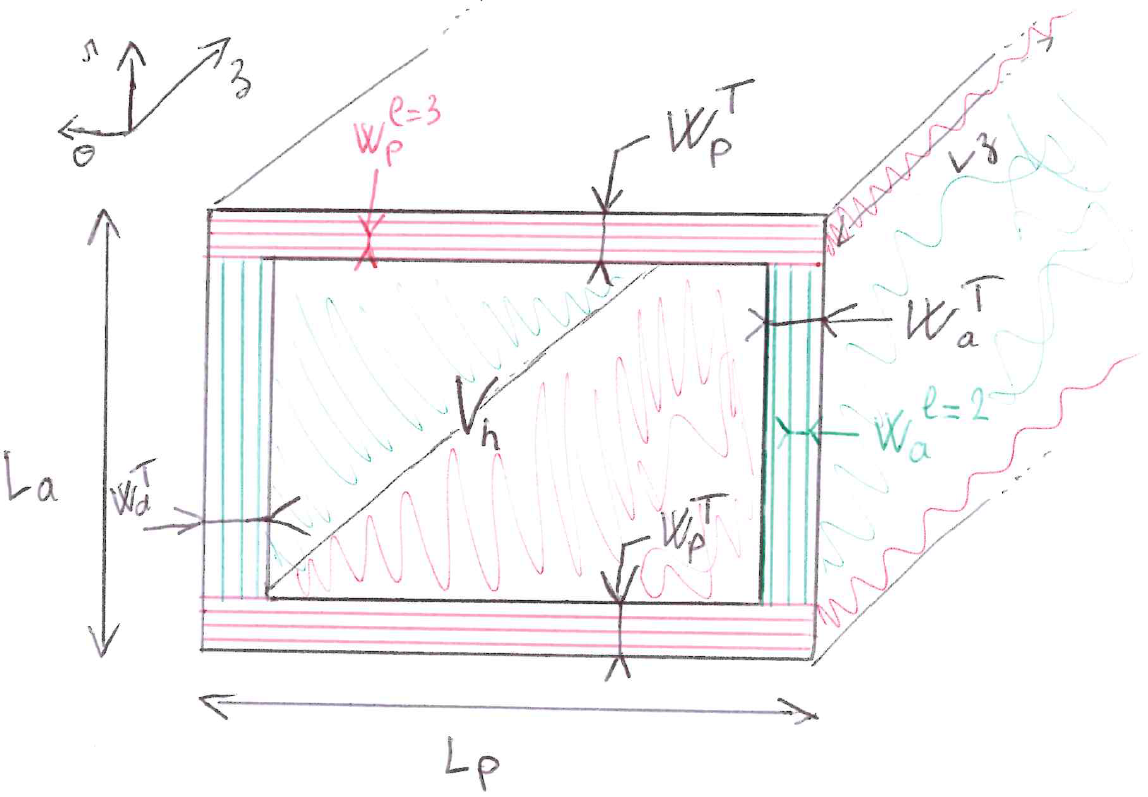
\includegraphics[width=0.5\textwidth]{schema.png}}
	\caption{Geometry and notations. The reference frame at the top left corner shows the link between the present geometry and the one of an actual cambial cell whose growth would be mainly along $r$.}
	\label{fig1}
\end{figure}
The geometry of the cambial cell is displayed in figure \ref{fig1}. Its total volume, $V^T$, is
\begin{equation}
	V^T = L_aL_pL_z,
\end{equation}
where $L_a$ is the length in the anticlinal direction, $L_p$ is the length in the periclinal direction, $L_z$ is the length in the longitudinal direction. $L_p$ and $L_z$ will be considered constant throughout this work.

Neglecting the end walls along $z$, the volume of water within the cell, $V_h$, is
\begin{equation}
	V_h = V^T - V_{wp}^T - V_{wa}^T,
\end{equation}
where $V_{wp}^T$ and $V_{wa}^T$ are the anticlinal and periclinal total wall volume, respectively. Taking the derivative of the previous equation gives
\begin{equation}
	\frac{{\rm d} V_h}{{\rm d} t}=L_pL_z\frac{{\rm d} L_a}{{\rm d} t} - \frac{{\rm d} V_{wa}^T}{{\rm d} t} - \frac{{\rm d} V_{wp}^T}{{\rm d} t}.
\end{equation}
Normalising the previous relation by $V_h$ leads to
\begin{equation}
	\frac{1}{V_h}\frac{{\rm d} V_h}{{\rm d} t}=\frac{L_pL_z}{V_h}\frac{{\rm d} L_a}{{\rm d} t} - \frac{1}{V_h}\frac{{\rm d} V_{wa}^T}{{\rm d} t} - \frac{1}{V_h}\frac{{\rm d} V_{wp}^T}{{\rm d} t}.
\end{equation}
Developping $L_pL_z/V_h $, the previous expression finally becomes
\begin{equation}\label{kinematic}
	\boxed{
	\frac{1}{V_h}\frac{{\rm d} V_h}{{\rm d} t}=\frac{1}{(1-2W_a^T/L_p)(L_a-2W_p^T)}\frac{{\rm d} L_a}{{\rm d} t} - \frac{1}{V_h}\frac{{\rm d} V_{wa}^T}{{\rm d} t} - \frac{1}{V_h}\frac{{\rm d} V_{wp}^T}{{\rm d} t}}.
\end{equation}
In the previous equation, we see that the volume of water in the cell increases with cell elongation and decreases with wall synthesis.

The total wall volumes can be computed as
\begin{equation}
	V_{wp}^T=2W_p^TL_pL_z,
\end{equation}
and
\begin{equation}
	V_{wa}^T=2W_a^TL_z(L_a-2W_p^T),
\end{equation}
where $W_p^T$ and $W_a^T$ are the periclinal and anticlinal total wall thicknesses.


\subsection{At the wall layer scale}
Walls are actually composed of several layers. For each layer, the wall volume is
\begin{equation}\label{periclinal_layer}
	V_{wp}^j=2W_p^jL_pL_z,
\end{equation}
with $j$ the layer number ($j \in [1;N_l^p]$, with $N_l^p$ the number of periclinal layers), for periclinal wall layers, and
\begin{equation}\label{anticlinal_layer}
	V_{wa}^i=2W_a^i L_z(L_a-2W_p^T),
\end{equation}
with $i$ the layer number ($i \in [1;N_l^a]$, with $N_l^a$ the number of anticlinal layers), for anticlinal wall layers. In previous equations, $V_{wp}^j$, $W_p^j$, $V_{wa}^i$ and $W_a^i$ are the periclinal layer volume and thickness, and the anticlinal layer volume and thickness, respectively. Note that all periclinal layers have the same length ($L_p$) and all anticlinal layers have the same length ($L_a-2W_p^T$).

Taking the derivative of Eq. (\ref{periclinal_layer}) leads to
\begin{equation}
	\frac{{\rm d} V_{wp}^j}{{\rm d} t}=2L_zL_p\frac{{\rm d} W_{p}^j}{{\rm d} t},
\end{equation}
which gives an equation for each periclinal layer thickness,
\begin{equation}
	\boxed{
	\frac{{\rm d} W_{p}^j}{{\rm d} t}=\frac{1}{2L_zL_p}\frac{{\rm d} V_{wp}^j}{{\rm d} t}}.
\end{equation}
Thus, because we assumed a constant $L_p$, $W_p$ only changes with periclinal wall synthesis.

Taking the derivative of Eq. (\ref{anticlinal_layer}) leads to
\begin{equation}
	\frac{{\rm d} V_{wa}^i}{{\rm d} t}=2L_z(L_a-2W_p^T)\frac{{\rm d} W_{a}^i}{{\rm d} t} +2W_a^iL_z\left(\frac{{\rm d} L_a}{{\rm d} t}-2\frac{{\rm d} W_p^T}{{\rm d} t}\right),
\end{equation}
which can then be reorganised to give an equation for each anticlinal wall layer thickness,
\begin{equation}\label{anticlinal_thickness}
	\boxed{
	\frac{{\rm d} W_{a}^i}{{\rm d} t}=\frac{1}{2L_z(L_a-2W_p^T)}\frac{{\rm d} V_{wa}^i}{{\rm d} t}  - \frac{W_a^i}{L_a-2W_p^T}\left(\frac{{\rm d} L_a}{{\rm d} t}-2\frac{{\rm d} W_p^T}{{\rm d} t}\right)}.
\end{equation}
The previous equation shows that each anticlinal layer will grow with wall synthesis and with the growth of the periclinal wall (this latter property being the direct consequence of the geometry presented in figure \ref{fig1}). The layer thickness will decrease with anticlinal wall elongation.

\subsection{Bridges between scales}
The relations between the total and layer volumes are
\begin{equation}
	V_{wp}^T=\sum_{j=1}^{j=N_l^p}V_{wp}^j, 
	\quad\text{and}\quad
	V_{wa}^T=\sum_{i=1}^{i=N_l^a}V_{wa}^i.
\end{equation}
In both walls, $i,j=1$ corresponds to the outermost/oldest wall layer. Similarly, the relations for the thicknesses are
\begin{equation}
	W_{p}^T=\sum_{j=1}^{j=N_l^p}W_{p}^j, 
	\quad\text{and}\quad
	W_{a}^T=\sum_{i=1}^{i=N_l^p}W_{a}^i.
\end{equation}
Taking the derivative of the previous expressions, we also have
\begin{equation}
	\frac{{\rm d} V_{wp}^T}{{\rm d} t}=\sum_{j=1}^{j=N_l^p}\frac{{\rm d} V_{wp}^j}{{\rm d} t}, 
	\quad\text{and}\quad
	\frac{{\rm d} V_{wa}^T}{{\rm d} t}=\sum_{i=1}^{i=N_l^a}\frac{{\rm d} V_{wa}^i}{{\rm d} t},
\end{equation}
for the wall volumes. Hence, the changes in total wall volumes are the sum of the volume changes of all the individual layers. Similarly, for wall thicknesses, we have
\begin{equation}
	\frac{{\rm d} W_{p}^T}{{\rm d} t}=\sum_{j=1}^{j=N_l^p}\frac{{\rm d} W_{p}^j}{{\rm d} t}, 
	\quad\text{and}\quad
	\frac{{\rm d} W_{a}^T}{{\rm d} t}=\sum_{i=1}^{i=N_l^a}\frac{{\rm d} W_{a}^i}{{\rm d} t}.
\end{equation}
\section{Water fluxes}
The changes in the volume of water inside the cell depends on the water fluxes:
\begin{equation}
	\frac{{\rm d} V_h}{{\rm d} t}=AK_h\left(P_{src} - \Pi_{src} -P + \Pi \right),
\end{equation}
where $A=2L_z(L_p+L_a)$ (neglecting water entry through end walls), $K_h$, $P_{src}$, $\Pi_{src}$, $P$ and $\Pi$ are the cylinder external area (m$^2$), the hydraulic conductivity (m/s/Pa), the pressure potential of the water source (Pa), the osmotic potential of water source (Pa), the cell turgor pressure (Pa) and the cell osmotic potential (Pa), respectively.
Dividing by $V_h$ further leads to
\begin{equation}
	\boxed{
		\frac{1}{V_h}\frac{{\rm d} V_h}{{\rm d} t}=\frac{AK_h}{V_h}\left(P_{src} - \Pi_{src} -P + \Pi \right)}.
\end{equation}
\section{Elongation rate}
The elongation rate of the anticlinal walls is
\begin{equation}
	\dot{\varepsilon}_a=\frac{1}{L_a-2W_p^T}\left(\frac{{\rm d} L_a}{{\rm d} t}-2\frac{{\rm d} W_p^T}{{\rm d} t}\right).
\end{equation}
Assuming ${\rm d} W_p^T/{\rm d} t=0$ one can identify its expression using Eq. (\ref{kinematic}):
\begin{equation}
	\boxed{
	\dot{\varepsilon}_a = \frac{1-W_a^T/L_p}{V_h}\left(\frac{{\rm d} V_h}{{\rm d} t} + \frac{{\rm d} V_{wa}^T}{{\rm d} t} +\frac{{\rm d} V_{wp}^T}{{\rm d} t} \right)},
\end{equation}
where the first term on the right hand side will be computed from the water fluxes, and the second term will depend on the wall synthesis dynamic.
Once the elongation rate is known, one can use it in different ways. First, one can use it to derive an equation for the cell length, i.e.,
\begin{equation}
	\boxed{
	\frac{{\rm d} L_a}{{\rm d} t}=\left(L_a-2W_p^T\right )\dot{\varepsilon}_a}.
\end{equation}
Secondly, it can be used to compute the evolution of the wall stresses in the anticlinal wall layers. Because of the geometry, all layers have the same elongation rate. If the rheology of the anticlinal wall layer material is described as a Bingham fluid, the elongation rate is related to the layer's stress, $\sigma_a^i$, as
\begin{equation}
	\dot{\varepsilon}_a=\frac{\left(\sigma_a^i-\sigma_Y\right)^+}{\mu}+\frac{1}{E}\frac{{\rm d} \sigma_a^i}{{\rm d} t},
\end{equation}
where $\sigma_Y$ is the wall layer yield stress (threshold for plastic deformation), $\mu$ is the wall layer viscosity, and $E$ is the wall layer Young's modulus. These three material properties are considered homogeneous across all layers (but this hypothesis could be relaxed in futur work). The $(x)^+$ notation is equivalent to ${\rm max} (x,0)$.
This equation can further be rearranged to obtain the stress changes for each wall layer, i.e.,
\begin{equation}
	\boxed{
	\frac{{\rm d} \sigma_a^i}{{\rm d} t}= E \dot{\varepsilon}_a- \frac{E\left(\sigma_a^i-\sigma_Y\right)^+}{\mu}}.
\end{equation}
This equation is valid for $i \in [1;N_l^a]$. If for any numerical reasons there are layers with $i>N_l^a$, this expression must be equal to 0. The initial stress value (at the layer creation) can be equal to 0, or to $\sigma_Y$, or to another custom value.

The mean anticlinal wall stress is related to the layers' stresses and thicknesses through
\begin{equation}
	\overline{\sigma_a}=\frac{\sum_i \sigma_a^i W_a^i}{\sum_i W_a^i}.
\end{equation}
\section{Mechanical equilibrium}
Cell turgor pressure and mean wall stresses are related through the following equilibrium conditions
\begin{equation}
	\overline{\sigma_a}=\frac{(P-P_{ext})L_p}{2W_a^T},
\end{equation}
\begin{equation}
	\overline{\sigma_p}=\frac{(P-P_{ext})L_a}{2W_p^T},
\end{equation}
where $P_{ext}$ is an external pressure applied on the walls. The first equation will be used to compute the turgor pressure, i.e.,
\begin{equation}
	P=\frac{2\overline{\sigma_a}W_a^T}{L_p} + P_{ext},
\end{equation}
and the second equilibrium condition will be used to compute the stress in periclinal walls.\\

\section{Wall layer synthesis (inspired by Friend \textit{et al.}, \textit{Nature com.}, 2022)}
Changes in wall layer volume are related to changes in mass, $M_{wa}^i$ (kg/cell), through $\rho_w$, the cell wall density (kg/m$^3$):
\begin{equation}
	\boxed{
		\frac{{\rm d} V_{wa}^i}{{\rm d} t}=\frac{1}{\rho_w}\frac{{\rm d} M_{wa}^i}{{\rm d} t}}.
\end{equation}
The same equation can be used for preclinal walls. With the modelling approach we used so far, the wall synthesis term is present in every cell wall layer. It could be used to represent a case where synthesis could still occur in old layers, in addition to the synthesis of new ones. As a first approximation, we will consider that wall synthesis occurs exclusively in the newest layer and is related to sugar availability through a Michaelis-Menten equation, i.e.,
\begin{equation}
	\boxed{
	\frac{{\rm d} M_{wa}^i}{{\rm d} t} = \begin{cases}
		0, & \text{if } i < N_l^a \\
		\frac{\Delta{M_{wa}^{max}}n_s/V_h}{n_s/V_h + K_m}, & \text{if } i = N_l^a
	\end{cases} \\}
\end{equation}

where $\Delta M_{wa}^{max}$ is the maximum speed of wall synthesis (kg/cell/s), $n_s$ is the sugar content (in mol) of the cell and $K_m$ is a kinetic constant (mol/m$^3$). A similar equation can be used for the periclinal wall layers, but for now we will asusme there is no synthesis in those layers, i.e.,
\begin{equation}
	\boxed{
		\frac{{\rm d} V_{wp}^j}{{\rm d} t}=\frac{1}{\rho_w}\frac{{\rm d} M_{wp}^j}{{\rm d} t}=0},
\end{equation}
for all periclinal layers. Note that the equations are implemented in their most general form so that in future development we can easily relax the different hypotheses made on wall synthesis.

The maximum speed of wall synthesis could further be related to water volume and temperature using a Bolztmann-Arrhenius equation,
\begin{equation}
	\boxed{
		\Delta M_{wa}^{max}=\omega V_h e^{\frac{E^a_w}{k}(1/T_0-1/T)}}.
\end{equation}
In the previous equation, $\omega$ is the normalised rate of cell-wall mass growth (kg/cell/s/m$^3$) at temperature $T_0$ (273.15 K), $E_w^a$ is an activation energy for wall building (eV), $k$ is Bolztmann's constant (eV/K) and $T$ is the actual temperature (K).

\section{Osmotic potential and sugar content}
If only one type of osmolytes is present, the cell osmotic potential is 
\begin{equation}
	\boxed{
		\Pi = \frac{n_s R_g T}{V_h}},
\end{equation}
where $R_g$ is the ideal gas constant. The evolution of the sugar content can be related to wall synthesis and other sugar fluxes through
\begin{equation}
	\boxed{
		\frac{{\rm d} n_s}{{\rm d} t}=-\frac{1}{M_s}\left(\sum_i\frac{{\rm d} M_{wa}^i}{{\rm d} t}+\sum_j\frac{{\rm d} M_{wp}^j}{{\rm d} t}\right) + f_s},
\end{equation}
where $M_s$ is the sugar molar mass (kg/mol), and $f_s$ is the sum of the sugar fluxes entering or leaving the cell.
Note that with the hypotheses we made on wall synthesis, this equation reduces to
\begin{equation}
		\frac{{\rm d} n_s}{{\rm d} t}=-\frac{1}{M_s}\frac{{\rm d} M_{wa}^{i=N_l^a}}{{\rm d} t} + f_s.
\end{equation}
 $f_s$ can be a constant, i.e., a constant sugar flux forced into the cell, or can be computed through a diffusion equation, i.e.,
\begin{equation}
	\boxed{
		f_s = \eta_s \left(C_s^{ext} - \frac{n_s}{V_h} \right)},
\end{equation}
with $\eta_s$ the sugar diffusion constant (m$^3$/s) and $C_s^{ext}$ the external osmotic concentration. This external osmotic concentration can then be used to simulate periods of low or high sugar availability. 
\section{Wall layer deposition dynamic}
New layer deposition occurs at a regular time interval (chosen by the user). In between these layer creations, wall matter is always deposited in the newest layer.

\section{Regulations}
A couple of regulations can be tried, the most obvious one is probably to keep a constant total wall thickness with time despite the deposition of new layers at each iteration. One can derive the equivalent of Eq. (\ref{anticlinal_thickness}) at the scale of the cell wall (it is the same equation with different superscipts),
\begin{equation}
		\frac{{\rm d} W_{a}^T}{{\rm d} t}=\frac{1}{2L_z(L_a-2W_p^T)}\frac{{\rm d} V_{wa}^T}{{\rm d} t}  - \frac{W_a^T}{L_a-2W_p^T}\left(\frac{{\rm d} L_a}{{\rm d} t}-2\frac{{\rm d} W_p^T}{{\rm d} t}\right).
\end{equation}
For a constant wall thickness, the left hand side is zero, and we get an expression for the total wall synthesis,
\begin{equation}
		\frac{{\rm d} V_{wa}^T}{{\rm d} t} = 2L_zW_a^T\left(\frac{{\rm d} L_a}{{\rm d} t}-2\frac{{\rm d} W_p^T}{{\rm d} t}\right).
\end{equation}
Wall synthesis only occuring in the last layer (or current iteration), one obtains
\begin{equation}
	\boxed{
	\frac{{\rm d} V_{wa}^{i=N_l^a}}{{\rm d} t} = 2L_zW_a^T\left(\frac{{\rm d} L_a}{{\rm d} t}-2\frac{{\rm d} W_p^T}{{\rm d} t}\right)},
\end{equation}
which will ensure a constant total wall thickness with a multilayered wall where new layers are deposited at each iteration. This will also stops wall synthesis when elongation stops.

Another regulation is the osmoregulation, that can be obtained by imposing
\begin{equation}
	\frac{{\rm d} n_s}{{\rm d} t} = \frac{n_s}{V_h}\frac{{\rm d} V_h}{{\rm d} t},
\end{equation}
which leads to 
\begin{equation}
	\frac{{\rm d} n_s}{{\rm d} t} = \frac{n_s}{V_h}\left(\frac{{\rm d} L_a}{{\rm d} t}(L_pL_z-2W_a^TL_z) -2L_z\frac{{\rm d} W_a^T}{{\rm d} t}(L_a-2W_p^T)\right).
\end{equation}
\end{document}